\documentclass[11pt]{article}

\usepackage[margin=1in]{geometry}
\usepackage{amsmath,amssymb}
\usepackage{graphicx}
\usepackage[colorlinks=true,linkcolor=blue,citecolor=blue,urlcolor=blue]{hyperref}
\usepackage{natbib}

\title{Evaporation Toward a Degenerate Horizon:\\
Islands, Asymptotics and the Horizonless Branch\\
of the Hayward Black Hole}

\author{Gracen Ownby}
\date{}

\begin{document}
\maketitle

\begin{abstract}
We study the late-stage evaporation of a Hayward-type regular black hole whose regularization scale is tied to the mass so that the core density is mass-independent, $\varepsilon^3=2GM\ell^2/c^2$. The metric has a critical mass $M^*=(3\sqrt3/4)\,\ell c^2/G$ at which its inner and outer horizons merge \citep{Hayward2006,KimNam2021}. Far from $M^*$ it reproduces Schwarzschild to fractional order $(\ell/M)^2$, so to a distant observer the object is an extremely time-dilated collapsed star. We make four points. First, the quasi-static (eternal black hole) approximation used in the island literature is justified along the evaporation: an adiabaticity parameter is of order $10^{-83}$ for a $10\,M_\odot$ hole, is small at $M^*$, and, with the near-extremal mass-loss law, vanishes as the endpoint is approached. Second, within the continuous semiclassical mass-loss law the transition at $M^*$ is never completed in finite time. The horizon area at $M^*$ is a fixed nonzero constant while the surface gravity vanishes, so the emission power scales as $\epsilon^2$ in the mass excess $\epsilon=M-M^*$ and $\epsilon\propto1/u$. This is the analogue for this metric of the unattainability of extremality known for charged black holes, and infinite evaporation times are known for regular black holes in general; it is not a new structural statement. The continuous law fails in a small window above $M^*$, where the emission of a single quantum or near-extremal quantum-gravity effects become important. Third, the island mechanism remains intact along the approach. The entropy plateau approaches, at leading order, the area value $3\pi\ell^2/G$, the leading term of the extremal Hayward island entropy of \citet{KimNam2021}; the extremal result is not the limit of the non-extremal one, and we do not resolve the subleading terms. Fourth, for $M<M^*$ the geometry has no horizon and supports no island, by two independent arguments: linear area growth near the point of maximal redshift, and a purity argument. For $M\gtrsim0.81\,M^*$ it also has a stable inner light ring, as a general theorem requires for smooth ultracompact objects satisfying the null energy condition; a test-scalar WKB calculation, cross-validated against a time-domain evolution, finds genuinely long-lived trapped modes there, consistent with the expectation that the horizonless configuration is not a stable endpoint. Whether general relativity coupled to standard matter can supply the core is treated in a companion paper.
\end{abstract}

\section{Introduction}
\label{sec:intro}

\citet{OppenheimerSnyder1939} showed that a collapsing dust cloud reaches the horizon in finite proper time while a distant observer sees the collapse proceed without ever quite completing. This observation underlies the ``frozen star'' picture of a black hole. The picture adopted here differs in emphasis: the collapse is not paused but slowed, so that the object remains, for an outside observer, a collapsing star whose progress is throttled by gravitational time dilation. Hawking radiation then acts as the exhaust that drives the object's evolution. As the object loses mass the time dilation relaxes, and the question is what happens at the end. We call the resulting long epoch of slowly relaxing time dilation \emph{Relativistic Sublimation}. The mathematical singularity of the classical solution is replaced by a finite-density core, as in the regular black holes of \citet{Bardeen1968} and \citet{Hayward2006}, so no singularity forms at any point of the history. The regularization is motivated by an appeal to a maximum density of the kind quantum degeneracy pressure might supply; the Horizon Quantum Mechanics framework \citep{CasadioGiugnoMicu2016} has been invoked in the same spirit. Whether standard matter can in fact supply such a core is a separate question, examined in the companion paper \citep{PaperB}. Nothing in the exterior analysis below depends on the answer, since the interior is causally screened by the horizon.

\paragraph{The physical picture.} In this picture the stellar-collapse sequence continues past the point where an event horizon would classically form. Degeneracy pressure persists at every stage but is never sufficient to halt the collapse, which is never truly static, only appearing frozen to a distant observer; beyond the classical horizon, protons and neutrons are expected to dissolve into quarks and gluons, whose degeneracy pressure is larger but still insufficient. An observer at the horizon finds the infall effectively completed, while a distant observer finds the external universe racing ahead. Matter beyond the horizon is not destroyed; it simply cannot be observed directly. As the object approaches the critical mass, gravity ceases to keep the local escape speed above $c$ and the extreme time dilation relaxes; the outermost shell is then expected to disperse gently, as an ordinary star would, rather than in a supernova. These statements describe the conceptual picture and are hypotheses of this framework, not results derived here; what is derived below concerns the metric, its evaporation, and the entropy of the radiation.

The distinctive endpoint of this model is the critical mass $M^*$ at which the horizons merge, so the natural questions concern the approach to it. Does the object reach $M^*$ in finite time? Does the quasi-static approximation used in the island literature hold all the way there? Does the entanglement-island mechanism that restores unitarity far from extremality survive as the horizon structure degenerates? And what does the geometry beyond the endpoint support? These are the questions of this paper.

\paragraph{Context.}
Whether evaporation is unitary was sharpened quantitatively by \citet{Page1993}, and entanglement islands \citep{Penington2019,AMMZ2019,AHMST2020,EngelhardtWall2015} are now the standard way to compute the fine-grained entropy of Hawking radiation. The island construction for an eternal Schwarzschild hole in four and higher dimensions is due to \citet{Hashimoto2020}. Islands for the Hayward metric, including its extremal case, were computed by \citet{KimNam2021}, and for Bardeen and Hayward spacetimes by \citet{Luongo2024}; near-extremal islands for a T-duality regular black hole have been studied by \citet{Anand2026}. There is also a broader literature on whether islands are generic to evaporating compact objects or a consequence of having an ordinary horizon. Work on fuzzball-inspired geometries with a stretched horizon \citep{AgeevZueva2026} found that island existence depends on the behavior of candidate extremal surfaces near the stretched cap, building on the ``blinking island'' effect for a reflecting boundary outside an eternal black hole \citep{AgeevArefevaRusalev2025}, and a Jackiw--Teitelboim de~Sitter study with timelike boundaries \citep{Rusalev2025} found islands persisting in one sector and failing to exist, by a clean nonexistence proof, in another.

A second body of work concerns the endpoint of evaporation near extremality, and it is extensive. For charged black holes the semiclassical evolution approaches the extremal state only asymptotically, in accordance with the unattainability of zero temperature \citep{SorkinPiran2001}, and it has been proposed that fully extremal configurations may be the asymptotic endpoint of black hole evolution \citep{DiFilippo2024}. For regular black holes with an inner horizon, the evaporation time is generically infinite \citep{CarballoRubio2018}, the final state is a critical remnant reached only in infinite time \citep{Bonanno2023}, and the possible global structures of such spacetimes have been classified in a model-independent way \citep{SuetoYoshino2026}. For the Hayward metric specifically, the thermodynamic picture, in which the temperature peaks and then falls to zero at a minimal-mass extremal configuration that leaves a remnant, was described by \citet{MehdipourAhmadi2016}; a related final-stage analysis through the generalized entropy has been given for rotating regular black holes \citep{Takeuchi2026}; and the renormalization-group-improved metric of \citet{BonannoReuter2000} has a mass-dependent core term and a Planck-scale critical mass, with evaporation argued to halt near it. Very close to extremality the continuous semiclassical description itself breaks down \citep{Preskill1991}: the emission of a single quantum can drive the object across extremality \citep{Gralla2026}, while the backreaction of a single Hawking quantum and Schwarzian quantum-gravity corrections substantially alter the emission rate \citep{Brown2024}. The point $M=M^*$ of the metric studied here shares with these cases the defining feature of coincident horizons; whether the near-extremal quantum analysis carries over is not addressed here.

\paragraph{What is and is not new.}
The metric, its critical mass, the identification of its parameter with a fixed length times the mass, the island entropy of its extremal case, the thermodynamic remnant picture, and the statement that extremality is approached only asymptotically, in infinite time, are all known (see above) and are treated here as baseline; we do not claim them. What this paper adds is more limited: the explicit mass-loss and horizon laws for this specific metric, which are direct corollaries of the general statements (Section~\ref{sec:massloss}); the adiabaticity analysis along the whole evaporation, including its scaling near the endpoint, which we have not found in the island literature; the one-sided, time-dependent island treatment at leading adiabatic order (Section~\ref{sec:islands}); and the analysis of the horizonless branch, including its island structure (Section~\ref{sec:horizonless}), whose light-ring structure follows from a general theorem and is verified explicitly. We do not address the instability of inner horizons under mass inflation \citep{PoissonIsrael1990,CarballoRubio2021,Bonanno2021}, which affects the $M>M^*$ interior irrespective of the source of the core.

\section{The Metric and Its Degenerate Point}
\label{sec:metric}

\subsection{A mass-independent core}

Take the Schwarzschild-like form with a regularized denominator, $f(r)=1-2GMr^2/[c^2(r^3+\varepsilon^3)]$. Computing the effective energy density implied by the metric through the Einstein tensor gives
\begin{equation}
\rho(r)=\frac{3M\varepsilon^3}{4\pi(\varepsilon^3+r^3)^2},\qquad \rho(0)=\frac{3M}{4\pi\varepsilon^3}.
\end{equation}
If $\varepsilon$ were held fixed and independent of $M$, the core density would grow without bound with $M$, contradicting the premise of a single universal maximum density. Requiring $\rho(0)$ to be independent of $M$ forces $\varepsilon^3\propto M$; we write
\begin{equation}
\varepsilon(M)^3=\frac{2GM\ell^2}{c^2},\qquad \rho(0)=\frac{3c^2}{8\pi G\ell^2},
\label{eq:eps-def}
\end{equation}
with $\ell$ a fixed length, taken at the Planck length in the numerical examples. The metric then becomes
\begin{equation}
ds^2=-f\,c^2dt^2+\frac{dr^2}{f}+r^2d\Omega^2,\qquad f=1-\frac{2GMr^2}{c^2\left(r^3+2GM\ell^2/c^2\right)},
\label{eq:metric}
\end{equation}
which is Hayward's metric exactly \citep{Hayward2006}: the combination $r^3+2GM\ell^2/c^2$ already carries this dependence in his original form. The identification of the Hayward parameter as $g=(2M\ell^2)^{1/3}$ with a fixed length $\ell$ appears explicitly in the literature \citep{MehdipourAhmadi2016}, following \citet{Frolov2016}; what is offered here is the density argument that motivates it. In units $G=c=1$ the effective source has $\rho\ge0$, $p_r=-\rho$ and $\rho+p_t\ge0$ everywhere, so the weak and null energy conditions hold and no negative-energy matter is required. Because $f(0)=1$ and $\rho(0)$ is finite for every $M$, the metric is regular at every mass, independently of the evaporation dynamics below.

\paragraph{Relation to other constructions.}
Mass-independence of the core is not peculiar to this motivation. A mass-dependent core term with a critical mass below which no horizon exists was already present in the renormalization-group-improved Schwarzschild metric of \citet{BonannoReuter2000}, which for a particular choice of parameters is a Hayward spacetime with an effective regularization length \citep{BorissovaCarballoRubio2026}, and a constraint linking the regularization scale to the mass function has been found from a dynamical-collapse viewpoint in exact solutions built from generalized polytropic matter \citep{KLV2026}. In a different direction, Hayward-, Bardeen- and Dymnikova-like regular black holes arise as exact vacuum solutions of quasi-topological gravities with infinite curvature towers \citep{BuenoCanoHennigar2025}, established in $D\ge5$ dimensions, with four-dimensional constructions developed since \citep{BuenoNonPoly2026,BorissovaCarballoRubio4D2026}, and with no matter source at all. The rationale offered here, a matter-supplied maximum density, is therefore one of several; see \citet{PaperB}. For a review of remnant scenarios and their difficulties see \citet{ChenOngYeom2015}.

\subsection{Horizon structure and the critical mass}

In units $G=c=1$ the horizons solve $r^3-2Mr^2+2M\ell^2=0$. For $M>M^*$ there are two positive roots $r_+>r_-$; at $M=M^*$ they coincide; for $M<M^*$ there is no positive root and the object has no horizon. The double root occurs at
\begin{equation}
M^*=\frac{3\sqrt3}{4}\,\ell\ \left(\frac{\ell c^2}{G}\ \text{in SI units}\right),\qquad r_h=\sqrt3\,\ell,\qquad A(M^*)=4\pi r_h^2=12\pi\ell^2,
\end{equation}
which is the known extremal mass of the Hayward metric \citep{Hayward2006,KimNam2021}. For $\ell$ at the Planck length, $M^*\approx2.83\times10^{-8}$~kg $\approx1.3\,m_P$. At this point the equation and its first radial derivative vanish while the second radial derivative and the mass derivative do not, the exact signature of two roots merging and annihilating. Writing $M=M^*+\epsilon$,
\begin{equation}
r_\pm(\epsilon)-r_h\approx\pm\frac{2\sqrt2\,3^{1/4}}{3}\sqrt{\ell\epsilon},\qquad \kappa(\epsilon)\approx c_\kappa\sqrt{\epsilon}\,\ell^{-3/2},\quad c_\kappa=\frac{2\sqrt2\,3^{1/4}}{9}\approx0.41,
\label{eq:fold}
\end{equation}
the standard square-root fold scaling, structurally identical to the merger of horizons at extremality in Reissner--Nordstr\"om. At $M^*$ the near-horizon geometry is $f\simeq(r-r_h)^2/(3\ell^2)$, so the AdS$_2$ radius equals $r_h=\sqrt3\,\ell$, the same structure as extremal Reissner--Nordstr\"om.

Far from $M^*$ the horizon can be expanded in the small parameter $\eta\equiv(\ell/M)^2$ (units $G=c=1$):
\begin{equation}
r_+=2M\left(1-\frac{\eta}{4}-\frac{\eta^2}{8}-\cdots\right),\qquad \frac{\kappa}{\kappa_{\rm Schw}}=1-\frac{\eta}{2}-\frac{3\eta^2}{8}-\cdots,
\end{equation}
with $\kappa_{\rm Schw}=1/4M$. For a $10\,M_\odot$ black hole with $\ell$ at the Planck length, $\eta\approx1.2\times10^{-78}$, so the modification is negligible for the entire $\sim10^{70}$-year evaporation history and becomes significant only as $M$ approaches $M^*$.

\subsection{Time dilation and Relativistic Sublimation}

The time-dilation factor for a static observer at radius $r$ is $\Gamma=d\tau/dt=\sqrt{f(r)}$, which reduces to the Schwarzschild $\sqrt{1-2GM/c^2r}$ up to the fractional correction of order $\eta$. To make the approach to the threshold visible over the enormous evaporation timeline, Fig.~\ref{fig:sublimation} plots $\Gamma$ against remaining mass on a logarithmic scale. The threshold $M^*$ marks where the object stops being a black hole in the technical sense; it does not mark where it stops being singular, which was never in question, since the core is regular at every mass.

\begin{figure}[htbp]
\centering
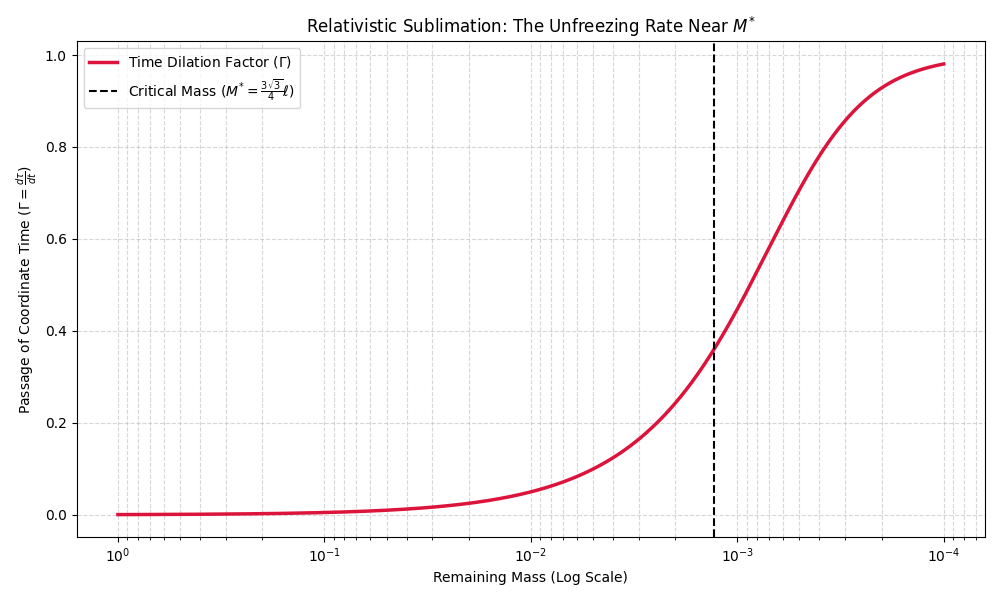
\includegraphics[width=0.85\textwidth]{sublimation_curve.png}
\caption{The time-dilation factor $\Gamma$ as a function of remaining mass (log scale, decreasing left to right), evaluated at the naive Schwarzschild radius for each mass. The dashed line marks the critical mass $M^*=\tfrac{3\sqrt3}{4}\ell$. For illustration $\ell$ is set several orders of magnitude larger than the Planck length so the transition is visible on the plotted scale; the qualitative shape, not this mass ratio, is the content of the figure.}
\label{fig:sublimation}
\end{figure}

\paragraph{Observational status.} Because the correction to Schwarzschild is of fractional size $\eta=(\ell/M)^2\sim10^{-78}$ for a stellar-mass black hole, the model is observationally indistinguishable from standard Schwarzschild general relativity for the entire evaporation lifetime of any astrophysical black hole, departing from it only in the final, sub-Planckian stage. This is consistent with, rather than in tension with, the dark central shadows seen by the Event Horizon Telescope \citep{EHT2019}: the model does not predict a persistently luminous shell of trapped matter at the horizon, since the radiation of infalling matter redshifts away on a light-crossing timescale ($r_s/c$, of order $10^{-4}$~s for a stellar-mass black hole) long before any effect of the regularized core becomes relevant. This is a qualitative consistency statement, not a fit to data.

\section{Mass Loss, Adiabaticity and the Approach to $M^*$}
\label{sec:massloss}

\subsection{Far from $M^*$: the Hawking law and the adiabaticity parameter}
\label{sec:adiabatic}

The Hawking power and temperature are
\begin{equation}
P=\frac{\hbar c^6}{15360\,\pi G^2M^2},\qquad T_H=\frac{\hbar c^3}{8\pi GMk_B}.
\end{equation}
For a $10\,M_\odot$ black hole, $P\approx9.0\times10^{-31}$~W and $T_H\approx6\times10^{-9}$~K. Since $T_H$ is far below the present CMB temperature, heat presently flows into the black hole and the horizon slowly grows; this reverses only once the CMB has redshifted below $T_H$. The mass loss obeys $dM/du=-P(M)$, integrating to the cube-root law $M(u)\propto(u_f-u)^{1/3}$ for $M\gg M^*$.

The island calculation of \citet{KimNam2021} models the black hole as an eternal, fixed-mass configuration coupled to a heat bath. This is a standard technique, but it needs justification for a genuinely evaporating object. We define the adiabaticity parameter as the fraction of the rest-mass energy radiated per light-crossing time of the horizon, $r_s/c$ with $r_s=2GM/c^2$,
\begin{equation}
\mathcal{A}(M)\equiv\frac{P(M)\,(r_s/c)}{Mc^2}=\frac{\hbar c}{7680\,\pi GM^2},
\label{eq:adiabaticity-param}
\end{equation}
so that quasi-static treatment is justified wherever $\mathcal{A}\ll1$. For a $10\,M_\odot$ black hole $\mathcal{A}\approx5\times10^{-83}$. Setting $\mathcal{A}=1$ gives the mass at which the approximation formally fails,
\begin{equation}
M_{\rm break}=\sqrt{\frac{\hbar c}{7680\,\pi G}}\approx1.4\times10^{-10}\ \mathrm{kg}\approx0.0064\,m_P,
\end{equation}
more than two orders of magnitude below $M^*$. Evaluating the Schwarzschild expression at the threshold gives $\mathcal{A}(M^*)\approx2.5\times10^{-5}$. This is a conservative figure, because the Schwarzschild law overestimates the emission near extremality, as the next subsection shows. The quasi-static approximation therefore holds across the evaporation, including the approach to $M^*$, and only fails at a mass below $M^*$, where the object has no horizon and the horizon-based island prescription no longer applies for a more basic reason.

\subsection{Near $M^*$: the corrected law}
\label{sec:corrected}

The Schwarzschild law cannot be continued to $M^*$. The surface gravity $\kappa(\epsilon)\propto\sqrt\epsilon$ vanishes continuously as $M\to M^*$, but the horizon \emph{area} does not: $A(M^*)=12\pi\ell^2$ is a fixed constant depending only on $\ell$. A Stefan--Boltzmann-type estimate for the emission power, $P\sim A(M^*)\,\kappa(\epsilon)^4$, gives
\begin{equation}
P(\epsilon)\;\propto\;\epsilon^2,
\end{equation}
which reproduces the Schwarzschild $M^{-2}$ law away from extremality (where $A\sim M^2$ and $\kappa\sim1/M$). Solving $d\epsilon/du=-P(\epsilon)\propto-\epsilon^2$ gives $\epsilon(u)\propto1/u$: \textbf{within this law, $M^*$ is approached only as $u\to\infty$ and never reached at finite retarded time}, the analogue for this metric of the unattainability of extremality \citep{SorkinPiran2001}. The general statement that the evaporation of a regular black hole with an inner horizon takes infinite time is established in \citet{CarballoRubio2018} and \citet{Bonanno2023}; the law derived here is its explicit form for this metric. The conclusion depends only on $P$ vanishing as a positive power of a continuously vanishing temperature, not on the coefficient, and is therefore robust to the details of the unmodeled greybody factors within the semiclassical regime. Continuing the cube-root law instead would predict a finite-time arrival at $M^*$; the two laws agree for $M\gg M^*$ and cross over where $\epsilon\sim M^*$.

\paragraph{Range of validity.}
The law $d\epsilon/du=-P(\epsilon)$ treats emission as a smooth flux. It ceases to be reliable once $\epsilon$ is comparable to the energy of a single emitted quantum, $\sim T_H(\epsilon)\propto\sqrt\epsilon$. With Eq.~\eqref{eq:fold}, this occurs for $\epsilon\lesssim\epsilon_c\sim(c_\kappa/2\pi)^2\ell^{-3}$ in Planck units, which for $\ell$ at the Planck length is a mass excess of order $10^{-2}$ Planck masses (a crude estimate). Two quantum effects act in that window, in different directions. Discreteness of emission can carry the object across $M^*$ in a single step, as in the analysis of \citet{Gralla2026} for charged black holes; Schwarzian corrections, where they apply, suppress the emission rate and can effectively halt the evaporation \citep{Preskill1991,IliesiuTuriaci2021,Brown2024}. We do not attempt to decide between them. Both questions treated below remain relevant: Section~\ref{sec:islands} describes the semiclassical approach, and Section~\ref{sec:horizonless} describes what the geometry supports if the object ends up on the other side of $M^*$.

\subsection{Apparent and event horizon dynamics}
\label{sec:horizons}

An analysis with the uncorrected Schwarzschild law would find the apparent-horizon branches $r_\pm(u)$ meeting at a sharp cusp, with formally divergent coordinate velocity $dr_\pm/du\sim1/\sqrt{u^*-u}$ at a finite merger time $u^*$. This is inconsistent with the previous subsection: $M^*$ is never reached at finite $u$, so no such $u^*$ exists. Using the corrected law, the chain rule gives
\begin{equation}
\frac{dr_+}{du}=\frac{dr_+}{d\epsilon}\frac{d\epsilon}{du}\;\propto\;\frac{1}{\sqrt\epsilon}\cdot(-\epsilon^2)\;=\;-\epsilon^{3/2}\;\longrightarrow\;0\quad(\epsilon\to0).
\label{eq:dr+du}
\end{equation}
The coordinate velocity of the apparent horizon vanishes rather than diverging: the horizon decelerates smoothly and freezes at $r_h$, with no cusp and no finite-time merger.

Writing the true (null) event horizon as $R_{\rm EH}(u)=r_+(u)+\delta(u)$, the exact outgoing null condition $dR/du=-f(R,M(u))/2$ linearizes to $\delta'(u)+\kappa(u)\delta(u)=-r_+'(u)$, with quasi-static solution $\delta\approx-r_+'(u)/\kappa(u)$. Far from $M^*$, in the ordinary Schwarzschild adiabatic regime, this gives the identity
\begin{equation}
\frac{\delta}{r_+}\approx2\,\mathcal{A}(M)\qquad(\text{far field}),
\label{eq:far-field-identity}
\end{equation}
which ties the event-horizon offset directly to the adiabaticity parameter of Section~\ref{sec:adiabatic}; it follows from $r_+\propto M$, $\kappa\propto1/M$, and $dr_+/dM=2$ all being functions of the single parameter $M$ in that regime, and is specific to it. Near $M^*$ the relevant small parameter is $\epsilon$, not $M$ (which is nearly constant, $\approx M^*$), so this far-field identity does not simply carry over; $\delta/r_+$ must be recomputed directly from its definition using the near-$M^*$ scalings already established, $\kappa(\epsilon)\propto\sqrt\epsilon$ and $dr_+/du\propto-\epsilon^{3/2}$ (Eq.~\eqref{eq:dr+du}), with $r_+\to r_h$ constant:
\begin{equation}
\frac{\delta}{r_+}=-\frac{r_+'(u)}{\kappa(u)\,r_+}\;\propto\;\frac{\epsilon^{3/2}}{\sqrt\epsilon}\;=\;\epsilon\qquad(\text{near }M^*).
\end{equation}
This still vanishes as $\epsilon\to0$, and does so faster than the comparison scale $\kappa'(u)/\kappa(u)^2\propto1/\sqrt u\propto\sqrt\epsilon$ (since $\epsilon<\sqrt\epsilon$ for small $\epsilon$): \emph{the adiabatic approximation improves, rather than degrades, approaching the asymptotic limit}, exactly as claimed, but via this direct near-$M^*$ computation rather than by substituting $\mathcal{A}(M)\propto\epsilon^2$ (itself correct as a scaling of $\mathcal{A}(M)$ by its definition, Eq.~\eqref{eq:adiabaticity-param}) into the far-field identity above, which does not hold in this regime and would give the wrong power of $\epsilon$. The delicate matched-asymptotic treatment that a sharp finite-time merger would require is unnecessary, because that scenario does not occur.

\section{Islands Along the Approach}
\label{sec:islands}

\subsection{The prescription and the static baseline}

The fine-grained entropy of the radiation is given by the quantum extremal surface prescription,
\begin{equation}
S=\min\,\mathrm{ext}\left[\frac{\mathcal{A}(\partial I)}{4G}+S_{\rm matter}(R\cup I)\right],
\end{equation}
where $I$ is the island and $R$ the radiation region \citep{EngelhardtWall2015,AMMZ2019}. For the eternal, two-sided Hayward black hole coupled to a bath, \citet{KimNam2021} find that after the Page time the island boundary sits just outside the horizon and the entropy saturates at
\begin{equation}
S_I=\frac{2\pi r_+^2}{G}+\left(\text{matter terms depending on }f\right),
\end{equation}
where the area term is universal, $2\pi r_+^2/G=2S_{\rm BH}$, the factor of two reflecting the two-sided eternal proxy, and the matter terms are their Eq.~(45) for the non-extremal Hayward metric. The matter terms include the ordinary bulk entanglement entropy of the fields between the horizon and the cutoff surface, present with or without an island. It is the saturation of the area term, not a bound on the full expression, that caps the radiation's entropy consistently with unitary evaporation rather than allowing the no-island entropy to grow without bound.

For the extremal Hayward metric, with $r_+=r_-=r_h=\sqrt3\,\ell$, \citet{KimNam2021} obtain, in our notation with $\mathcal{N}$ the number of fields carrying the radiation (their central charge $c$) and $b$ the location of the distant observer,
\begin{equation}
S_I=\frac{\pi r_h^2}{G}+\frac{\mathcal{N}}{12}\log\!\left(\frac{144\pi^2r_h^8(b-r_h)^2(2b+r_h)}{(\mathcal{N}G)^2(2b^3+r_h^3)}\right),
\label{eq:KN-extremal}
\end{equation}
which is finite. They emphasize that this extremal result is not the extremal limit of the non-extremal one. They also identify the role of the regular core: for the extremal Reissner--Nordstr\"om black hole the no-island entropy is infinite because $f(0)$ diverges, and the island boundary is driven to the curvature singularity, where the semiclassical approximation is invalid; in the regular Hayward metric $f(0)=1$ and neither problem arises. For non-extremal black holes the singularity never enters the calculation, so the regularization is not needed there.

\subsection{A time-dependent, one-sided treatment}

Adapting the static formula to a genuinely time-dependent conformal factor requires the analogue of the Kruskal coordinate for a slowly evolving surface gravity, $U(u)=-\exp(-\mathcal{K}(u))/\kappa(u)$ with $\mathcal{K}(u)\equiv\int\kappa(u')\,du'$, which reduces to the standard construction when $\kappa$ is constant. Direct computation gives
\begin{equation}
\frac{dU}{du}=e^{-\mathcal{K}(u)}\left[1+\frac{\kappa'(u)}{\kappa(u)^2}\right],
\end{equation}
where the correction term, evaluated near $M^*$ directly from $\kappa(\epsilon)\propto\sqrt\epsilon$ and $d\epsilon/du\propto-\epsilon^2$ (Section~\ref{sec:corrected}), scales as $\kappa'(u)/\kappa(u)^2\propto\sqrt\epsilon\to0$ — the same comparison scale identified in Section~\ref{sec:horizons}, not the far-field identity $2\mathcal{A}(M)$ of Eq.~\eqref{eq:far-field-identity}, which does not carry over to this regime. The resulting entropy at leading adiabatic order is the static expression with $e^{\kappa u}\to e^{\mathcal{K}(u)}$, correct up to this same controlled, and here vanishing, error. Extremizing for a physically one-sided island (area $4\pi r_a^2$, not the factor-of-two two-sided proxy) drives the island to within $O(\mathcal{N}G/r_+)$ of the horizon and gives the single-copy area term $\pi r_+^2/G$ at leading order, the appropriate checkpoint against the static result.

\subsection{The plateau at the endpoint}

Since the adiabaticity parameter vanishes as $u\to\infty$ rather than growing, the island mechanism continues to operate, with ever-improving accuracy, into the asymptotic limit. The horizon radius approaches $r_h=\sqrt3\,\ell$, so the fine-grained entropy plateau approaches
\begin{equation}
S_*=\frac{\pi r_h^2}{G}=\frac{3\pi\ell^2}{G},
\end{equation}
the leading term of Eq.~\eqref{eq:KN-extremal}, a finite value set entirely by the regularization scale. This holds at leading order in $1/G$ only. In the eternal, two-sided setting, \citet{KimNam2021} show that the extremal result is not the limit of the non-extremal one, whose matter term contains a piece that diverges logarithmically as $r_+\to r_-$, and that the plateau differs by a factor of two between the non-extremal case ($2S_{\rm BH}$) and the extremal case ($S_{\rm BH}$). Our one-sided treatment does not remove this subtlety, which concerns the subleading terms and the order of limits, and which we do not resolve.

We also use the area functional $A/4G$ throughout, as \citet{KimNam2021} do. For regular black holes whose thermodynamic entropy differs from $A/4G$, as happens when the regularization arises from a modified gravitational action, the plateau value would change, and for a T-duality regular black hole it has been argued that the island functional should instead be built from the first-law entropy \citep{Anand2026}. We do not resolve this choice. \textbf{Within the semiclassical regime, and at the level of the approximations stated, the evaporation of this model is information-safe without the object becoming horizonless.}

\subsection{Energetics of the terminal stage}

At $M=M^*$, with $\ell$ at the Planck length, the remnant mass is approximately the Planck mass, $m_P\approx2.176\times10^{-8}$~kg, and its rest energy is $E=m_Pc^2\approx1.95\times10^9$~J, roughly the energy of a concentrated lightning strike. A Bekenstein-bound estimate shows that a burst of this energy, confined to a region of order the Planck length, can carry at most a handful of bits, many orders of magnitude short of the $\sim10^{79}$ bits of entanglement entropy that must be accounted for over the evaporation of a $10\,M_\odot$ progenitor. The resolution of unitarity in this model therefore does not rest on the terminal energy release encoding the missing information. It rests on the generalized-entropy argument above, in which information is returned gradually, with the entropy curve turning over near the Page time, long before the terminal stage. The terminal energy release is a calculable feature of the model, but a minor byproduct of the regularization.

\section{The Horizonless Branch}
\label{sec:horizonless}

Section~\ref{sec:corrected} shows that the semiclassical evaporation does not cross $M^*$. But the continuous law fails near $M^*$, and a quantum effect could carry the object across. We therefore ask what the geometry supports for $M<M^*$, treating the question as a formal one about the geometry alone.

\subsection{Geometry}

For $M<M^*$ the horizon equation has no positive root, $f(r)>0$ everywhere, and the object has no horizon. The point of maximal redshift, the minimum of $f$, is at
\begin{equation}
r_{\min}(M)=2^{2/3}M^{1/3}\ell^{2/3},\qquad f(r_{\min})=1-(M/M^*)^{2/3},
\end{equation}
which is strictly positive for any $M>0$. Unlike a wormhole throat, this is not a minimum of the areal radius (that minimum is the smooth regular center at $r=0$), only a minimum of the redshift factor. That $r_{\min}$ and $r=0$ are different points is what makes the existence of islands in this regime a question worth checking rather than assuming.

\subsection{Why no island forms}

Testing for an island with the natural analogue of the static calculation, a radiation region $R$ extending from a distant observer to $r_{\min}$ and a candidate island occupying $[0,r_{\min}]$: the two diagnostics below are not logically independent evidence for the same conclusion, but one argument in two steps, worth stating both ways because each clarifies something the other does not.

The candidate island together with $R$ exhausts the \emph{entire} spatial slice, since no horizon remains to hide a separate region behind. Following the nonexistence argument of \citet{Rusalev2025}: if the global state on this slice is pure, the matter entanglement entropy of ``everything'' is trivially constant, its derivative with respect to the island's location is identically zero, and the extremization of generalized entropy over candidate island boundaries reduces entirely to the area term, with no compensating matter-entropy term able to produce a critical point. \emph{This is the step that does the actual logical work}: it is what licenses treating the area term in isolation at all, which would not otherwise be justified (the matter term is not generically negligible). Having reduced the problem to the area term alone, its behavior is exactly the question addressed by the general criterion of \citet{AgeevZueva2026} for horizonless geometries: whether a stable island can form near a point of maximal redshift depends on whether the area of nearby candidate extremal surfaces grows linearly or quadratically with proper distance. Since $r_{\min}>0$ and $dA/dr=8\pi r\neq0$ for any $r>0$ (not a special property of $r_{\min}$), the area grows \emph{linearly} everywhere, which generically makes any candidate surface a local maximum, not minimum, of generalized entropy, ruling out an extremum.

\textbf{Islands do not exist in the horizonless regime of this metric, however the object comes to be there.} This rests on purity doing the reduction and the area-growth criterion then applying cleanly to what is left, not on two independent lines of evidence happening to agree.

\subsection{A stable inner light ring}

A further caveat concerns the horizonless configuration itself. A general theorem states that smooth, ultracompact solutions formed from the collapse of matter obeying the null energy condition must have at least two light rings, one of them stable \citep{CunhaBertiHerdeiro2017}, and stable light rings have been argued to trigger nonlinear instabilities. The horizonless metric here is smooth and satisfies the null energy condition, so a stable inner light ring is expected (the continuation of regular black holes, Hayward's included, to horizonless ultracompact stars with inner and outer light rings is the subject of \citealt{CarballoRubio2022}), and we verify it explicitly for this mass-dependent family: the function $f/r^2$ has a local minimum, in addition to the unstable outer light ring, for $0.81\,M^*\lesssim M<M^*$, lying at $r\simeq1.73$--$1.77\,\ell$ for $M$ between $0.95\,M^*$ and $M^*$, just outside the point of minimal $f$. For Bardeen-type families interpolating between regular black holes and horizonless objects, compact horizonless configurations have been found to support long-lived modes tied to a stable photon sphere \citep{Franzin2024}, and nonlinear evolutions of ultracompact bosonic stars show that the light-ring instability drives them to migrate to non-ultracompact configurations or to collapse to black holes, typically within about $10^3$ light-crossing times unless the well is very shallow \citep{Cunha2023}. Here the well is not shallow: near $M^*$ the potential $f/r^2$ falls from its outer maximum, about $0.02\,\ell^{-2}$, to nearly zero at the inner minimum. This suggests that the horizonless configuration near $M^*$ is unlikely to be a stable endpoint, although the results cited concern other systems. We compute the trapped-mode spectrum of this metric directly below.


\subsection{The trapped-mode spectrum}
\label{sec:trapped}

A stable light ring generically traps wave packets, and the associated modes are the standard diagnostic for the nonlinear instability just described \citep{CardosoLongLived2014}. We compute this spectrum for a massless, minimally coupled test scalar field on the horizonless metric. A test field, rather than the coupled gravitational perturbation of the actual matter source, is used because \citet{PaperB} shows that the perturbative response of that source is not established; the scalar calculation is the standard proxy in this literature, and through the eikonal correspondence between wave propagation and null geodesics it captures the light-ring trapping mechanism responsible for the effect, independently of the spin of the field.

Separating $\Phi=(\psi(r)/r)Y_{lm}e^{-i\omega t}$ and passing to the tortoise coordinate $dx=dr/f(r)$, defined here by $x(0)=0$ (there is no horizon, so $x$ is finite and monotonic on $r\in[0,\infty)$), the wave equation reduces to the Regge--Wheeler form
\begin{equation}
\frac{d^2\psi}{dx^2}+\left[\omega^2-V_l(r)\right]\psi=0,\qquad V_l(r)=f(r)\left[\frac{l(l+1)}{r^2}+\frac{f'(r)}{r}\right],
\label{eq:RWpotential}
\end{equation}
with regularity at the center, $\psi\sim r^{l+1}$ as $r\to0$, and a purely outgoing wave at infinity. For $M<M^*$ in the window of Section~\ref{sec:horizonless}, $V_l$ diverges at $r=0$ (the ordinary centrifugal barrier), falls to a local minimum at the stable light ring, rises to a local maximum at the unstable one, and falls to zero at infinity: a well separated from the exterior by a barrier, with three real turning points $r_1<r_2<r_3$ for any $\omega^2$ between the extrema.

We locate the trapped-mode frequencies with the standard three-turning-point WKB method used for ultracompact objects \citep{CardosoLongLived2014}: Bohr--Sommerfeld quantization of the well fixes the real part,
\begin{equation}
\int_{r_1}^{r_2}\frac{\sqrt{\omega_R^2-V_l(r)}}{f(r)}\,dr=\left(n+\tfrac12\right)\pi,\qquad n=0,1,2,\dots,
\end{equation}
and the Gamow tunneling formula gives the decay rate,
\begin{equation}
\omega_I\approx-\frac{1}{T}\exp\!\left[-2\int_{r_2}^{r_3}\frac{\sqrt{V_l(r)-\omega_R^2}}{f(r)}\,dr\right],\qquad T=2\int_{r_1}^{r_2}\frac{dr}{f(r)\sqrt{\omega_R^2-V_l(r)}},
\end{equation}
$T$ being the classical round-trip time in the well. We validated this against a direct time-domain evolution of Eq.~\eqref{eq:RWpotential} (finite-difference, with the same regularity condition at $r=0$ and an absorbing outer boundary) for $l=2$, $M=0.90\,M^*$: the late-time signal at fixed $r$ oscillates at $\omega_R=0.4298\,\ell^{-1}$ against the WKB value $0.4303\,\ell^{-1}$ (0.1\% difference), and its envelope decays at rate $3.08\times10^{-3}\,\ell^{-1}$ against the WKB value $2.33\times10^{-3}\,\ell^{-1}$, a factor of 1.3, consistent with the known accuracy of leading-order WKB at low $l$ \citep{CardosoLongLived2014}.

\begin{table}[htbp]
\centering
\begin{tabular}{ccccc}
\hline
$M/M^*$ & $l$ & $\mathrm{Re}(\omega)\,\ell$ & $Q=\mathrm{Re}(\omega)/2|\mathrm{Im}(\omega)|$ & $\tau=1/|\mathrm{Im}(\omega)|$ \ [$\ell/c$] \\
\hline
$0.90$ & $1$ & $0.277$ & $4.2\times10^{1}$ & $3.0\times10^{2}$ \\
$0.90$ & $2$ & $0.430$ & $9.2\times10^{1}$ & $4.3\times10^{2}$ \\
$0.90$ & $4$ & $0.732$ & $1.2\times10^{3}$ & $3.1\times10^{3}$ \\
$0.95$ & $1$ & $0.200$ & $8.9\times10^{2}$ & $8.9\times10^{3}$ \\
$0.95$ & $2$ & $0.309$ & $1.7\times10^{4}$ & $1.1\times10^{5}$ \\
$0.99$ & $1$ & $0.090$ & $1.3\times10^{6}$ & $3.0\times10^{7}$ \\
\hline
\end{tabular}
\caption{Fundamental ($n=0$) trapped-mode frequency, quality factor and $e$-folding lifetime, for the multipoles and masses least dependent on the eikonal approximation. $Q$ grows rapidly with $l$ and as $M\to M^*$: the well deepens relative to the barrier as $M^*$ is approached (at $l=5$, the gap between the well bottom and barrier top grows from $0.28\,\ell^{-2}$ at $M=0.90\,M^*$ to $0.70\,\ell^{-2}$ at $M=0.99\,M^*$).}
\label{tab:trapped}
\end{table}

Even at $l=1$, the least trustworthy multipole for a leading-order WKB treatment, $Q\gg1$ and $\tau$ is hundreds of light-crossing times; both grow rapidly with $l$ and with proximity to $M^*$, reaching values too large to be physically meaningful (Table~\ref{tab:trapped} stops at the multipoles where this is not yet the case). Two caveats limit what this establishes. First, at large $l$ the relevant length scale $r/l$ approaches and then undercuts $\ell$, the scale at which the classical field treatment used here is not trustworthy in the first place; the largest entries in the table should be read as confirming the trend, not as physical predictions. Second, this is a test-field calculation, not the coupled gravitational perturbation of the true matter source, which \citet{PaperB} shows is not yet identified; the qualitative conclusion is expected to survive that gap, since it follows from the light-ring structure of the geometry itself rather than from the specific field considered, but we have not verified this. Within these limits, the low-$l$, numerically validated modes already show genuinely long-lived trapping, consistent with the general expectation that the horizonless configuration is not a quiet endpoint.

\section{Discussion}
\label{sec:disc}

\subsection{What is established}

The two halves of the analysis are complementary. Within the continuous semiclassical law, the evaporation never crosses into the regime where the horizonless analysis would matter. The object approaches $M^*$ asymptotically, the quasi-static approximation improves along the approach, and the island mechanism remains, indeed becomes more reliably, intact, with the plateau approaching a finite value set by the regularization scale. In the small window above $M^*$ where the continuous law fails, both halves are needed: if a quantum effect carries the object across $M^*$, the horizonless analysis says what the geometry supports there, namely no island, for two structurally independent reasons that do not depend on how the configuration was reached. The information-safety conclusion is therefore secure only within the semiclassical regime. Beyond it, the question turns on the quantum treatment of the final approach and on how a horizonless object purifies the earlier radiation, neither of which this paper provides.

\subsection{Relation to the singularity theorems and mass inflation}

This model does not challenge Penrose's theorem \citep{Penrose1965}, which remains a rigorous result given its hypotheses. Static regular black holes of the Hayward type evade its conclusion not by violating the null energy condition, which holds everywhere, but through a different premise: the inner Cauchy horizon of these geometries violates the theorem's global-hyperbolicity requirement \citep{Borde1997}. Inner horizons of this kind are, however, subject to the mass-inflation instability \citep{PoissonIsrael1990}, and whether regular cores survive it is actively debated \citep{CarballoRubio2021,Bonanno2021}; the present paper does not address that instability. Separately, the dynamical evaporation relies on the standard fact that Hawking radiation involves a local violation of the null energy condition in the semiclassical stress tensor near the horizon, without which the horizon could not shrink under the classical area theorem. This holds equally for singular and regular black holes.

\subsection{A lesson for remnant scenarios}

Within the semiclassical regime, the resolution of unitarity in this model does not come from anything special about a horizonless endpoint, which does not support the island mechanism at all. It comes from the island mechanism operating throughout an asymptotic approach in which the object remains a (vanishingly cool, but technically still radiating) black hole. Any remnant scenario that relies on unitarity being restored specifically \emph{after} horizon loss should be regarded with the caution these results suggest, since the horizonless configuration would then have to restore it by some mechanism other than islands.

\subsection{Open items}

Several points are left open. The subleading terms of the plateau and the order of limits at the extremal point are unresolved. The choice between the area functional and a first-law entropy for regular black holes is unresolved. Whether the near-extremal quantum analysis of \citet{Brown2024} carries over to this geometry depends on the matter content of the near-horizon throat and is untested. The perturbation spectrum of the horizonless branch has been computed only at the test-scalar, WKB level (Section~\ref{sec:trapped}); the coupled gravitational spectrum of the true matter source is not yet accessible, pending the closure problem of \citet{PaperB}. The source of the regular core, and whether general relativity coupled to standard matter can supply it, are the subject of the companion paper \citep{PaperB}, whose results do not affect the exterior analysis here.

\section{Conclusion}

The picture developed here is of a black hole as a long-lived, extremely time-dilated collapsed star that evaporates according to the Hawking law while retaining a finite-density core. It reproduces Schwarzschild general relativity to extraordinary precision, to fractional order $(\ell/M)^2$, for essentially its whole evaporation lifetime, and departs from it only as the mass approaches the critical value $M^*=(3\sqrt3/4)\,\ell c^2/G$ at which the outer and inner horizons merge. Within the semiclassical regime the object approaches this degenerate horizon only asymptotically, the quasi-static approximation underlying the island calculation improves along the approach, and the fine-grained entropy of the radiation is capped at a finite plateau set by the regularization scale, consistent with unitary evaporation without a horizonless endpoint. If a quantum effect carries the object across $M^*$, the resulting horizonless geometry supports no island and has a stable inner light ring, so unitarity cannot be restored there by the island mechanism and the configuration is unlikely to be a stable endpoint. Much of the endpoint picture, namely the asymptotic approach, the remnant and the finite extremal entropy, is established in the literature cited above. The contribution of this paper is to assemble it for a single explicit metric, to verify the adiabatic validity of the eternal-black-hole approximation along the whole evaporation, and to analyze the horizonless branch.

\bibliographystyle{plainnat}
\bibliography{references}

\end{document}
